





\documentclass[
	% -- opções da classe memoir --
	12pt,				% tamanho da fonte
	openright,			% capítulos começam em pág ímpar (insere página vazia caso preciso)
	oneside,			% para impressão em recto e verso. Oposto a oneside
	a4paper,			% tamanho do papel. 
	% -- opções da classe abntex2 --
	%chapter=TITLE,		% títulos de capítulos convertidos em letras maiúsculas
	%section=TITLE,		% títulos de seções convertidos em letras maiúsculas
	%subsection=TITLE,	% títulos de subseções convertidos em letras maiúsculas
	%subsubsection=TITLE,% títulos de subsubseções convertidos em letras maiúsculas
	% -- opções do pacote babel --
	english,			% idioma adicional para hifenização
	french,				% idioma adicional para hifenização
	spanish,			% idioma adicional para hifenização
	brazil				% o último idioma é o principal do documento
	]{abntex2}




% Pacotes básicos 
\usepackage{lmodern}			% Usa a fonte Latin Modern			
\usepackage[T1]{fontenc}		% Selecao de codigos de fonte.
\usepackage[utf8]{inputenc}		% Codificacao do documento (conversão automática dos acentos)
\usepackage{indentfirst}		% Indenta o primeiro parágrafo de cada seção.
\usepackage{color}				% Controle das cores
\usepackage{graphicx}			% Inclusão de gráficos
\usepackage{microtype} 			% para melhorias de justificação
\usepackage{amsmath}			% lib para equacoes
\usepackage{svg}
%\usepackage{float}
\usepackage[T1]{fontenc}
\usepackage{listings}
\usepackage{tikz}
\usepackage{caption}
\usepackage{url}

\usepackage{titlesec}
\newcommand{\sectionbreak}{\clearpage}
\usepackage{hyperref}

\usetikzlibrary{shapes.geometric, arrows}

\tikzstyle{startstop} = [rectangle, rounded corners, 
minimum width=3cm, 
minimum height=1cm,
text centered, 
draw=black, 
fill=red!30]

\tikzstyle{io} = [trapezium, 
trapezium stretches=true, % A later addition
trapezium left angle=70, 
trapezium right angle=110, 
minimum width=3cm, 
minimum height=1cm, text centered, 
draw=black, fill=blue!30]


\tikzstyle{process} = [rectangle, 
minimum width=3cm, 
minimum height=1cm, 
text centered, 
text width=3cm, 
draw=black, 
fill=orange!30]

\tikzstyle{decision} = [diamond, 
minimum width=3cm, 
minimum height=1cm, 
text centered, 
draw=black, 
fill=green!30]
\tikzstyle{arrow} = [thick,->,>=stealth]



\definecolor{dkgreen}{rgb}{0,0.6,0}
\definecolor{gray}{rgb}{0.5,0.5,0.5}
\definecolor{mauve}{rgb}{0.58,0,0.82}

\lstset{frame=tb,
  language=Python,
  aboveskip=3mm,
  belowskip=3mm,
  showstringspaces=false,
  columns=flexible,
  basicstyle={\small\ttfamily},
  numbers=none,
  numberstyle=\tiny\color{gray},
  keywordstyle=\color{blue},
  commentstyle=\color{dkgreen},
  stringstyle=\color{mauve},
  breaklines=false,
  breakatwhitespace=false,
  upquote=true,
  tabsize=3
}

% Pacotes adicionais, usados apenas no âmbito do Modelo Canônico do abnteX2

\usepackage{lipsum}				% para geração de dummy text



% Pacotes de citações
\usepackage[num, backend=biblatex]{abntex2cite}	% Citações padrão ABNT
\usepackage[brazilian,hyperpageref]{backref}	 % Paginas com as citações na bibl

 
% CONFIGURAÇÕES DE PACOTES

% Configurações do pacote backref
% Usado sem a opção hyperpageref de backref
\renewcommand{\backrefpagesname}{Citado na(s) página(s):~}
% Texto padrão antes do número das páginas
\renewcommand{\backref}{}
% Define os textos da citação
\renewcommand*{\backrefalt}[4]{
	\ifcase #1 %
		Nenhuma citação no texto.%
	\or
		Citado na página #2.%
	\else
		Citado #1 vezes nas páginas #2.%
	\fi}%
% ---



% ---
% Informações de dados para CAPA e FOLHA DE ROSTO
% ---
\titulo{Robô omnidirecional de 3 rodas}
\autor{Daniel Ermelino Carvalho \\ Lucas Pereira Lima}
\local{Brasil}
\data{2024}
\orientador{Marcelo Bender Perotoni}
\instituicao{%
  Universidade Federal do ABC
  \par
  CECS
  \par
   Engenharia de Instrumentação, Automação e Robótica}
\tipotrabalho{Trabalho de graduação}
% O preambulo deve conter o tipo do trabalho, o objetivo, 
% o nome da instituição e a área de concentração 
\preambulo{Trabalho apresentado ao curso de engenharia de instrumentação,
automação e robótica da Universidade Federal do ABC como requisito parcial para
obtenção do título de bacharel em Engenharia de Instrumentação, Automação e 
Robótica.}



% Configurações de aparência do PDF final

% alterando o aspecto da cor azul
\definecolor{blue}{RGB}{5,5,180}

% informações do PDF
\makeatletter
\hypersetup{
     	%pagebackref=true,
		pdftitle={\@title}, 
		pdfauthor={\@author},
    	pdfsubject={\imprimirpreambulo},
	    pdfcreator={LaTeX with abnTeX2},
		pdfkeywords={abnt}{latex}{abntex}{abntex2}{trabalho acadêmico}, 
		colorlinks=true,       		% false: boxed links; true: colored links
    	linkcolor=blue,          	% color of internal links
    	citecolor=blue,        		% color of links to bibliography
    	filecolor=magenta,      		% color of file links
		urlcolor=blue,
		bookmarksdepth=4
}
\makeatother


% Posiciona figuras e tabelas no topo da página quando adicionadas sozinhas
% em um página em branco. Ver https://github.com/abntex/abntex2/issues/170
\makeatletter
\setlength{\@fptop}{5pt} % Set distance from top of page to first float
\makeatother



% Possibilita criação de Quadros e Lista de quadros.
% Ver https://github.com/abntex/abntex2/issues/176

\newcommand{\quadroname}{Quadro}
\newcommand{\listofquadrosname}{Lista de quadros}

\newfloat[chapter]{quadro}{loq}{\quadroname}
\newlistof{listofquadros}{loq}{\listofquadrosname}
\newlistentry{quadro}{loq}{0}

% configurações para atender às regras da ABNT
\setfloatadjustment{quadro}{\centering}
\counterwithout{quadro}{chapter}
\renewcommand{\cftquadroname}{\quadroname\space} 
\renewcommand*{\cftquadroaftersnum}{\hfill--\hfill}

\setfloatlocations{quadro}{hbtp} % Ver https://github.com/abntex/abntex2/issues/176


% Espaçamentos entre linhas e parágrafos 


% O tamanho do parágrafo é dado por:
\setlength{\parindent}{1.3cm}

% Controle do espaçamento entre um parágrafo e outro:
\setlength{\parskip}{0.2cm}  % tente também \onelineskip


% compila o indice
\makeindex


\renewcommand{\bibname}{Bibliografia}


% Início do documento
\begin{document}


\include{abntex2-modelo-include-comandos}

% Seleciona o idioma do documento (conforme pacotes do babel)
%\selectlanguage{english}
\selectlanguage{brazil}

% Retira espaço extra obsoleto entre as frases.
\frenchspacing 


% ELEMENTOS PRÉ-TEXTUAIS

	% Capa
	\imprimircapa

	% Folha de rosto
	% (o * indica que haverá a ficha bibliográfica)
	\imprimirfolhaderosto

	% inserir lista de ilustrações
	\pdfbookmark[0]{\listfigurename}{lof}
	\listoffigures*
	\cleardoublepage

	% inserir lista de quadros
	\pdfbookmark[0]{\listofquadrosname}{loq}
	\listofquadros*
	\cleardoublepage

	% inserir lista de abreviaturas e siglas
	\begin{siglas}
		\item[ABNT] Associação Brasileira de Normas Técnicas
		\item[abnTeX] ABsurdas Normas para TeX
	\end{siglas}

	% inserir o sumario
	\pdfbookmark[0]{\contentsname}{toc}
	\tableofcontents*
	\cleardoublepage


% ELEMENTOS TEXTUAIS
\textual

	% Introdução (exemplo de capítulo sem numeração, mas presente no Sumário)

	\input{chapters/introducao.tex}

	\chapter{Objetivos}

\subsection*{Gerais}
Este trabalho tem como objetivos gerais avaliar a viabilidade da utilização de 
um robô omnidirecional de três rodas controlado por microcontrolador para 
atuação em ambiente interno.

\subsection*{Específicos}
Deseja-se realizar a construção de um robô a partir de diversos componentes 
(motor, microcontrolador, rodas, driver, chassi, entre outros), e também 
implementar rotina de controle remoto que permita a operação do robô a partir de 
comandos via smartphone.

	
\chapter{Metodologia}



\section{Modelagem do robô}

Um veículo omnidirecional de 3 rodas no contexto deste trabalho é um robô
holonômico capaz de se mover em translação e rotação simultanea e
independentemente \cite{mobile_manipulator_robot}. Sua geometria se 
baseia em rodas equidistantes em uma circunferência, com 120° de separação entre
si, tangenciando o circulo formado pelos centros geométricos das rodas,
como demonstrado \autoref{modelo_geometrico}.

\begin{figure}[ht]
	\centering
	\caption{Diagrama do modelo matemático do robô}
	\label{modelo_geometrico}
	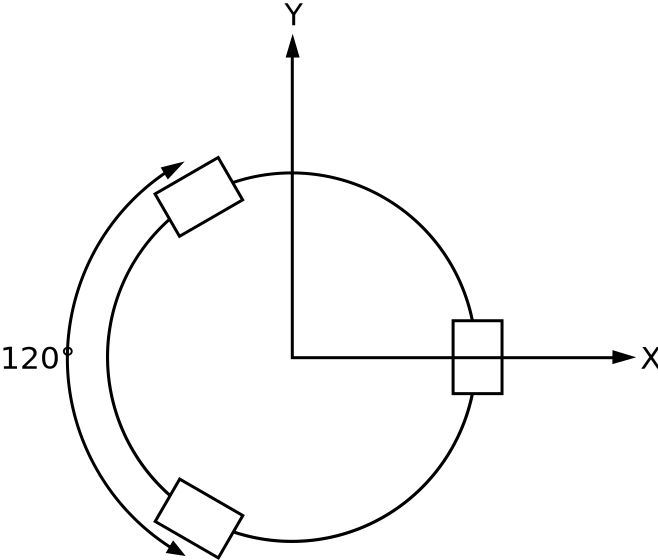
\includegraphics{figures/model}
	\caption*{FONTE: Própria}
\end{figure}

Robôs omnidirecionais tais como esse são particularmente úteis porque permitem
 maior manobrabilidade e eficiência, a um custo de maior complexidade na sua
 construção e controle. \cite{dynamical_models_for_omni_directional_robots}

\subsection{Modelagem Cinemática - Dedução da matriz por cinemática direta}

$\overrightarrow{V}$ é o vetor de velocidade linear do robô, $V_{w1}$, $V_{w2}$,
$V_{w3}$ são as velocidades lineares das rodas 1,2,3. 
$\omega $ é a velocidade angular do robô a partir do seu centro geométrico.
$L$ é a distância entre o centro de geométrico da roda e o centro de geométrico
do robô.

\begin{figure}[ht]
	\centering
	\caption{Diagrama do modelo matemático do robô, com valores dos ângulos das
	rodas}
	\includegraphics[width=0.8\textwidth]{figures/digram_model_dedution}
	\caption*{FONTE: Própria}
\end{figure}

\begin{equation}
    \begin{split}
        \overrightarrow{V}_{l} = 
        \overrightarrow{V}_{w1}
        + \overrightarrow{V}_{w2}
        + \overrightarrow{V}_{w3}
    \end{split}
\end{equation}

\begin{equation}
    \begin{split}
        \overrightarrow{\omega} = 
        \frac{\vert\overrightarrow{V}_{w1}\vert}{L}
        + \frac{\vert\overrightarrow{V}_{w2}\vert}{L}
        + \frac{\vert\overrightarrow{V}_{w3}\vert}{L}
    \end{split}
\end{equation}

\begin{gather*}
        V_{l} \angle \theta =  
        V_{w1} \angle \left(-\frac{\pi}{2}\right) 
        + V_{w2} \angle \left(\frac{2\pi}{3}-\frac{\pi}{2}\right) 
        + V_{w3} \angle \left(\frac{4\pi}{3}-\frac{\pi}{2}\right) 
\end{gather*}
\begin{gather*}
    V_{l} \cos{ \theta } + jV_{l} \sin{\theta} =  \\
    V_{w1} \cos{ \left(-\frac{\pi}{2}\right)} + jV_{w1} \sin{ \left(-\frac{\pi}{2}\right) } \\
    + V_{w2}  \cos{ \left(\frac{\pi}{6}\right) } + jV_{w2}  \sin{ \left(\frac{\pi}{6}\right) }  \\
    + V_{w3} \cos{ \left(\frac{5\pi}{6}\right) } + jV_{w3}  \sin{ \left(\frac{5\pi}{6}\right) } 
\end{gather*}

\begin{equation*}
    \begin{split}
        \omega = 
        \frac{V_{w1}}{L}
        + \frac{V_{w2}}{L}
        + \frac{V_{w3}}{L}
    \end{split}
\end{equation*}

\begin{gather}
	\begin{bmatrix} V\cdot \cos{\theta} \\  V\cdot \sin{\theta} \\  \omega \end{bmatrix}
	=
	\begin{bmatrix}
		\cos{\left(-\frac{\pi}{2}\right)} & \cos{\left(\frac{\pi}{6}\right)} & \cos{\left(\frac{5\pi}{6}\right)} \\
		\sin{\left(-\frac{\pi}{2}\right)} & \sin{\left(\frac{\pi}{6}\right)} & \sin{\left(\frac{5\pi}{6}\right)} \\
		\frac{1}{L} & \frac{1}{L} & \frac{1}{L}
	\end{bmatrix}
	\cdot
	\begin{bmatrix} V_{w1} \\  V_{w2} \\  V_{w3} \end{bmatrix}
\end{gather}

Matriz da cinemática direta:
\begin{gather}
	\begin{bmatrix}
		\cos{\left(-\frac{\pi}{2}\right)} & \cos{\left(\frac{\pi}{6}\right)} & \cos{\left(\frac{5\pi}{6}\right)} \\
		\sin{\left(-\frac{\pi}{2}\right)} & \sin{\left(\frac{\pi}{6}\right)} & \sin{\left(\frac{5\pi}{6}\right)} \\
		\frac{1}{L} & \frac{1}{L} & \frac{1}{L}
	\end{bmatrix}
	=
	\begin{bmatrix}
		0 & \sqrt{3}/2 & -\sqrt{3}/2 \\
		-1 & 1/2 & 1/2  \\
		1/L & 1/L & 1/L
	\end{bmatrix}
\end{gather}
Matriz inversa:
\begin{gather}
	\label{matriz_inversa}
	\begin{bmatrix} V_{w1} \\  V_{w2} \\  V_{w3} \end{bmatrix}
	=
	\begin{bmatrix}
		0 & -2/3 & L/3 \\
		1/\sqrt{3} & 1/3 & L/3\\
		-1/\sqrt{3} & 1/3 & L/3
	\end{bmatrix}
	\cdot
	\begin{bmatrix} V\cdot \cos{\theta} \\  V\cdot \sin{\theta} \\  \omega \end{bmatrix}
\end{gather}
A equação \eqref{matriz_inversa} é a matriz de cinemática do robô.
As entradas são o vetor velocidade linear e a velocidade angular do robô, e as
saídas são as velocidades lineares de cada uma das rodas.

Desconsiderando a velocidade angular, é possível observar os vetores velocidades
das rodas e o vetor velocidade linear do robô na \autoref{simulacao}, que
foi gerada por meio de simulação em Python. O código fonte da simulação está
disponível em \url{https://github.com/dcarve/tg-robot/tree/master/simulation/vectors_simulation/src}.

\begin{figure}[ht]
	\centering
	\caption{Simulação dos vetores}
	\includegraphics[width=0.7\textwidth]{figures/simulacao}
	\caption*{FONTE: Própria}
	\label{simulacao}
\end{figure}

O algoritmo da matriz inversa de cinemática transcrito em C, pode ser encontrado no apêndice \ref{matriz_cinematica_c}

\section{Roda Omnidirecional}

A roda omnidirecional aparece em vários modelos na literatura, tais como no design de J. Graboweicki em 1919
\cite{patent_US1305535A} e o de Josef Blumrich em 1972 \cite{patent_US3789947A}. A roda consiste de rolos
perpendiculares à  sua direção de giro, cuja presença tem como efeito conferir à roda a capacidade de se locomover em
qualquer direção no seu plano. Essa capacidade é o que confere aos robôs aqui discutidos suas características
holonômicas, uma vez que as restrições de movimento a que eles estão sujeitos está normalmente atrelada à construção dasrodas \cite{TAKAHASHI}.

\begin{figure}[h]
	\centering
	\caption{Modelo de uma Roda Omnidirecional}
	\includegraphics[width=0.5\textwidth]{figures/omniwheel}
    \caption*{FONTE: https://www.vexrobotics.com/omni-wheels.html}
\end{figure}

A relação entre velocidade linear e angular da roda é dada por:

\[V_{w1} = \omega_{w1}\cdot r \] 

em que $V_{w}$ é velocidade linear da roda, $r$ o raio da roda, $\omega_{w} $ e é a velocidade angular da roda.

Uma variação da roda omnidirecional é a roda mecanum, criada por Bengt Ilon \cite{patent_US3876255A} - 
a diferença fundamental entre elas é a construção dos rolos ligados à estrutura central  -
os quais, no caso da roda mecanum, são posicionados a 45°.

\subsection{Obtenção da roda omnidirecional}

Inicialmente foram compradas roda prontas, fabricas fora do território nacional, por meio de importação.
Mas o mesmo modelo pode ser encontrado sendo vendido no Brasil.
O modelo adquirido inicialmente possui diametro de 58mm, largura de 26mm e possui um acoplamento para eixo de 4mm de diametro.
Essas dimensões foram adquadas nos primeiros testes de contrução do robô enquanto se estava usando motores DC,
mas quando o projeto passou a usar motores de passo Nema 17, as rodas não eram mais compatíveis com o eixo e as dimensões dos motores.
(A mudança de tipos de motores será discutida na seção sobre motores).

\begin{figure}[h]
	\centering
	\caption{Roda omnidirecional usada inicialmente}
	\includegraphics[width=0.5\textwidth]{figures/roda_china.png}
    \caption*{FONTE: https://rapidroboticsaustralia.com/products/58mm-nylon-omni-directional-wheel-4mm-hub}
\end{figure}

A mudança de requisitores para as rodas levou a criar um design próprio e fabricado com impressoa 3d,
parafusos sextavado de M3, e reutilizando os rolamentos das rodas de 58mm.
As novas rodas possuem 69mm de diametro e 27mm de largura, fabricadas com filamento PLA.

\begin{figure}[h]
	\centering
	\caption{Processo de desing da nova roda - AutoCAD}
	\includegraphics[width=0.9\textwidth]{figures/roda_processo_desing_passo1}
    \caption*{FONTE: Própria}
\end{figure}

\begin{figure}[h]
	\centering
	\caption{Estudo e testes do design da nova roda}
	\includegraphics[width=0.9\textwidth]{figures/estudo_roda}
    \caption*{FONTE: Própria}
\end{figure}

\begin{figure}[h]
	\centering
	\caption{Desing final - Solidworks}
	\includegraphics[width=0.9\textwidth]{figures/roda_processo_desing_passo2}
    \caption*{FONTE: Própria}
\end{figure}

\begin{figure}[h]
	\centering
	\caption{Desing final - Preparação para impressão}
	\includegraphics[width=0.9\textwidth]{figures/roda_processo_desing_passo3}
    \caption*{FONTE: Própria}
\end{figure}

\begin{figure}[h]
	\centering
	\caption{Montagem da roda}
	\includegraphics[width=0.9\textwidth]{figures/roda_processo_desing_passo4}
    \caption*{FONTE: Própria}
\end{figure}

\section{Microcontrolador e IDE} \label{microcontrolador_ide}

\subsection{Microcontrolador}

Microcontroladores são circuitos integrados compactos desenvolvidos para governar
uma operação específica em um sistema embarcado. No contexto da aplicação deste
trabalho, o uso de um microcontrolador é fundamental para se obter o controle
desejado de trajetória e posicionamento do robô.

Duas placas de microcontrolador o BluePill e ESP32 Devkit v1 foram testadas.
Ambas possuem processadores de 32bits e podem ser alimentadas através dos pinos
de 5V e 3.3V, e também através do connector micro-USB-B.

A escolha dessas placas foi motivada pelo seu custo de aquisição e pelos
componentes e opções de comunicação disponíveis. A placa BluePill já havia sido
adquirida anteriormente ao desenvolvimento deste projeto, de modo que seu uso
não incorreria em custos adicionais. Semelhantemente, a escolha da placa ESP32
Devkit V1 também foi motivada também pelo custo, mas a capacidade de integração
por Bluetooth mostrou-se particularmente relevante neste contexto, tornando a
placa uma boa candidata para esta aplicação. Tal integração integração será
discutida nas seções a seguir.

A \autoref{precos_placas} compara a faixa de preço entre as principais
placas de desenvolvimento disponíveis para compra em território nacional.

\begin{table}[ht]
	\centering
	\caption{Comparação de preços entre as placas de desenvolvimento \label{precos_placas}}
	 \begin{tabular}{|c|c|}
		\hline
		\textbf{Placa de desenvolvimento} & \textbf{Faixa de preço em R\$} \\ \hline
		BluePill (STM32F103C8T6) &  23 - 49 (já adquirido anteriormente) \\ \hline
		ESP32 DevKit V1  &  40 - 80   \\ \hline
		Arduino Due R3 &  320 - 470   \\ \hline
		Nodemcu v3 ESP8266 & 22 - 35   \\ \hline
		Raspberry pi pico (1, 2, W, H)  & 36 - 66  \\ \hline
	\end{tabular}
	\caption*{FONTE: Própria}
\end{table}

Os preços aqui apresentados têm como base os valores praticados pelas principais
lojas nacionais de componentes eletrônicos online:
\begin{itemize}
	\item https://www.rsrobotica.com.br/
	\item https://www.robocore.net/
	\item https://www.makerhero.com/
	\item https://www.iot-robotica.com.br/
	\item https://www.ardurobotica.com.br/
	\item https://curtocircuito.com.br/
	\item https://www.saravati.com.br/
	\item https://www.a2robotics.com.br/
	\item https://www.ardurobotica.com.br/
	\item https://www.casadarobotica.com/
\end{itemize}



\subsubsection{BluePill - STM32F103C8}

A placa BluePill embarca o microcontrolador STM32F103C8.
"STM32" é uma família de microcontroladores de 32-bits fabricados pela
ST-Microelectronics. O processador empregado nessa família é o ARM Cortex-M3
\cite{cortex_m3}, baseado em arquitetura Harvard, com 64Kbs de memória flash.

De acordo com o livro \textit{Discovering the STM32 Microcontroller}
\cite{stm_doc} e a documentação colaborativa do projeto STM32-base.org
\cite{stm32_base_org}, a placa possui também 7 timers, 2 ADCs, e 9 interfaces de
comunicação, incluindo I2C,  USART, SPI, e USB 2.0.

A placa STM32 apresenta 7 pinos que suportam canais de PWM de 5V, e outros 8
canais de 3.3V, e pode ser alimentada via microUSB de 5V. Existem 3 grupos de
pinos: $P_{A}$, $P_{B}$ e $P_{C}$. Os pinos $P_{A}$ vão de $P_{A0}$ 
a $P_{A15}$, os $P_{B}$ vão de $P_{B0}$ a $P_{B15}$, e $P_{C}$, com apenas 3
pinos, de $P_{C13}$, $P_{C14}$ e $P_{C15}$.
A relação geral dos pinos pode ser melhor observada na figura 
\autoref{stm32f103c8_pinout}.

\begin{figure}[ht]
	\centering
	\caption{Diagrama de pinos do STM32F103C8}
	\includegraphics[width=1.0\textwidth]{figures/stm32f1_pinout}
	\caption*{FONTE: Sistemas Microprocessados - Apostila com práticas e foco nos processadores ARM CORTEX \cite{apostila_microprossados}}
    \label{stm32f103c8_pinout}
\end{figure}

O gravador ST-LINK v2 é o padrão para carregar projetos no microcontrolador.
Esse gravador, cuja versão original (\autoref{stlinkv2_original}) é fabricada
pela ST-Microelectronics, pode ser encontrada em uma versão paralela a menores
custos online (\autoref{stlinkv2_cheap}). Contudo, as versões paralelas, por
serem produzidas por fabricantes diversos, e por vezes não claramente indicados 
na descrição do produto. Por essa razão, pode haver variação na relação de
pinos (\autoref{stlinkv2_cheap_pin_diff}).

É possível modificar o firmware da placa STM32F103C8 para permitir o
carregamento de projetos via USB, contudo tal esse procedimento
é nativamente suportado ST-Microelectronics, tornando necessário o uso de
ferramentas de terceiros - por vezes, mesmo projetos de código aberto não mais
ativamente mantidos \cite{stm32duino_bootloader}.
A conexão micro-USB-B ainda funciona como uma comunicação serial, podendo ser
usada como uma porta serial para fins de \textit{debugging}. Contudo, utilizá-la
ao mesmo tempo que o ST-link pode danificar o microcontrolador, já que o
regulador recebe 5V da entrada USB e disponibiliza 3.3V volts, ao mesmo tempo
em que mas 3.3V também estão sendo disponibilizados diretamente a partir do
gravador ST-link.

\begin{figure}[ht]
	\centering
	\caption{St-Link V2 original fabricado pela ST-Microelectronics \cite{st_link_v2}}
	\includegraphics[width=0.5\textwidth]{figures/stlinkv2_original}
	\caption*{FONTE: ST-Microelectronics - ST-Link V2}
    \label{stlinkv2_original}
\end{figure}


\begin{figure}[ht]
	\centering
	\caption{St-Link V2 paralelo de fabricação desconhecida \cite{stlinkv2_cheap_ref}}
	\includegraphics[width=0.5\textwidth]{figures/stlinkv2_cheap}
	\caption*{FONTE: https://www.achavevirou.com.br/gravador-st-link-v2-para-stm32-e-stm8}
    \label{stlinkv2_cheap}
\end{figure}


\begin{figure}[htb]
	\centering
	\caption{St-Link V2 paralelo e o problema da não padronização de pinos}
	\includegraphics[width=0.5\textwidth]{figures/stlinkv2_cheap_pin_diff}
	\caption*{
		FONTE: Adaptado de https://universal-solder.ca/st-link-v2-usb-programmer-debugger/
		e https://www.achavevirou.com.br/gravador-st-link-v2-para-stm32-e-stm8
	}
    \label{stlinkv2_cheap_pin_diff}
\end{figure}

No restante desse trabalho, todas as menções a "STM32" referem-se à placa
BluePill.


\subsubsection{ESP32 Devkit v1}

A placa ESP32 Devkit v1, de fabricação da DOIT.am, possui o microcontrolador
ESP32-WROOM-32E (\autoref{esp32_pinout}), fabricado pela Espressif Systems.
A série ESP32 foi lançada em 2016 \cite{anuncio_esp32}, e possui arquitetura de
32 bits. Ela tem se tornado popular por possuir opções com integração Bluetooth
e WiFi. O microcontrolador ESP32-WROOM-32E possui um processador dual core
ESP32-D0WD-V3 \cite{esp32_wroom_32e_datasheet}, com frequência máxima de 240MHz,
WiFi 2.4Ghz de até 150Mbps e Bluetooth 4.2. Embora a placa tenha 48 GPIOs, elas
estão endereçadas em apenas 25 pinos. Entre os periféricos, existem 15 canais
ADC, 2 interfaces UART, 2 canais DAC, 25 PWM, uma interface de SPI, I2C e I2S,
e 9 interfaces de toque capacitivo
\cite{esp32_reference_2} \cite{esp32_reference}.

\begin{figure}[ht]
	\centering
	\caption{Diagrama de pinos da placa ESP32 Devkit v1}
	\includegraphics[width=1.0\textwidth]{figures/esp32_pinout}
	\caption*{FONTE: Adaptado https://lastminuteengineers.com/esp32-pinout-reference/}
	\label{esp32_pinout}
\end{figure}

Artigos contribuídos pela comunidade online sobre a placa ESP32 Devkit v1 
\cite{esp32_reference_2} \cite{esp32_reference} sugerem que nem todos os 25
pinos podem ser livremente utilizados - alguns possuem limitações de uso de
acordo com o periférico em uso. A \autoref{esp32_pinout_ref} resume as
recomendações de uso do pinos. Diferentemente da placa STM32, é possível
carregar projetos na placa ESP32 Devkit v1 nativamente via USB.

\begin{figure}[ht]
	\centering
	\caption{Recomendação de uso dos pinos da placa ESP32 Devkit v1}
	\includegraphics[width=0.35\textwidth]{figures/esp32_pinout_ref}
	\caption*{FONTE: Adaptado https://lastminuteengineers.com/esp32-pinout-reference/}
	\label{esp32_pinout_ref}
\end{figure}

No restante deste trabalho, todas as menções a "ESP32" referem-se à placa
ESP32 Devkit v1.


\subsection{IDE}

\subsubsection{Atollic TrueSTUDIO}

\begin{figure}[ht]
	\centering
	\caption{Interface Atollic}
	\includegraphics[width=0.8\textwidth]{figures/atollic}
	\caption*{FONTE: Sistemas Microprocessados - Apostila com práticas e foco nos processadores ARM CORTEX \cite{apostila_microprossados}}
\end{figure}

A IDE padrão empregada para programar projetos para a placa STM32 é o TrueSTUDIO,
distribuído pela Atollic, que foi adquirida pela ST-Microelectronics em 2017.
Trata-se de um software livre para programar em C/C++, criado com base na
plataforma Eclipse, e que possui todas as funções necessárias para o
desenvolvimento com a placa STM32, tais como edição, compilação e debugging.
Uma de seus principais vantagens é a ausência de limitações quanto ao tamanho
do projeto, o que o torna ideal para trabalhos profissionais. A IDE TrueSTUDIO
deixou de receber atualizações em 2017, depois da aquisição da Atollic pela 
ST-Microelectronics \cite{apostila_microprossados}.


\subsubsection{Arduino IDE}

Criado para ser a IDE das placa de desenvolvimento Arduino, a primeira
versão da Arduino IDE foi criada em 2005 \cite{arduino_id_history}.
Suas versões mais populares disponíveis para o público são 1.0.6 e 1.8. 
A versão 1.8 foi lançada em 2016 e recebeu atualizações até 2021, 
e a versão 2.0.0 foi lançada em 2022 \cite{arduino_tag_2}.

\begin{figure}[ht]
	\centering
	\caption{Interface Arduino}
	\includegraphics[width=0.9\textwidth]{figures/arduino}
	\caption*{FONTE: Própria}
\end{figure}

\subsection{Escolha do microcontrolador e IDE}

\subsubsection{IDE}

Devido a complicações nas configurações de múltiplas saídas de PWM com o 
TrueSTUDIO, optou-se por usar Arduino como alternativa. Um obstáculo a essa
alternativa é que o Arduino não é compatível com STM32 nativamente. Esse
empecilho pode ser contornado por meio do uso do projeto Arduino\_STM32
\cite{arduino_stm32}, de Roger Clark. O projeto contem os arquivos na linguagem
C necessários para viabilizar o uso do hardware da placa STM32 com a Arduino IDE.
Até o momento de escrita deste trabalho, o projeto era compatível apenas com a
versão 1.8 da Arduino IDE.

Transposto o obstáculo inicial à sua utilização, a Arduino IDE do Arduino 
logo se demonstrou uma opção mais viável e flexível, tanto pela vasta lista
bibliotecas disponibilizadas por contribuidores voluntários quanto pela grande
quantidade de documentações de projetos independentes.

A Arduino IDE também é compatível com a placa ESP32 por meio do uso da
biblioteca arduino-esp32 \cite{arduino_esp32}, disponibilizada e mantida
pela Espressif Systems.

\subsubsection{Microcontrolador}

Durante o desenvolvimento deste projeto, algumas dificuldades tornaram a
utilização da placa STM32 inviável. Entre esses dificuldades, destacam-se a
impossibilidade do uso da porta micro-USB-B da placa STM32 simultaneamente ao
gravador ST-link, bem como a impossibilidade de se manter o módulo HC-05 ligado
durante o processo de gravação na placa. Esta última dificuldade ocasionou a
perda de dois módulos HC-05, dado que, no tocante aos pinos de comunicação serial,
quaisquer comportamentos diferentes do padrão durante a gravação de um podem
ocasionar dano ao módulo (o que de fato ocorreu, uma vez que o módulo HC-05 foi
deixado conectado à placa STM32 durante a gravação múltiplas vezes), e aquela
foi causa de dano à própria placa STM32.

Tais dificuldades no uso da placa STM32 com relação à conexão via micro-USB-B e
o uso do módulo HC-05 demonstraram que a placa ESP32 era uma melhor candidata 
para uso neste trabalho. A troca de placas não acarretou mudanças significativas
em outras partes do projeto, dado que a placa ESP32 apresenta integração
com Bluetooth nativamente e suporta gravação de projetos via micro-USB-B
para gravação ao mesmo tempo em que a comunicação serial é utilizada para
\textit{debugging}, e também que foi possível continuar a utilizar a Arduino IDE
por meio da biblioteca arduino-esp32.

\section{Controle e comunicação com o microcontrolador}

\lipsum[1]

\section{Motores}  \label{secao_motores}

\subsection{Motores DC}


Um motor DC é essencialmente uma máquina elétrica de corrente contínua, que
converte energia elétrica de corrente contínua em energia mecânica. Máquinas
elétricas de corrente contínua são mais fácies de se controlar (quando
comparadas a máquinas de corrente alternada) e oferecem uma grande faixa de
velocidades \cite{Maquinas_eletricas}. Devido a essas características, tornam-se
boas candidatas para uso em eletrônica e robótica, uma vez que é viável
utilizá-las com com baterias. Para controlar a velocidade de um motor, é
necessário o uso de um encoder, que converte o sinal de posição em um valor
mensurável de velocidade angular, e também um driver, que permite a
microcontroladores controlarem a atuação do motor.

\subsubsection{Encoder magnético}

	Encoders magnéticos são um tipo de encoder rotacional que utiliza sensores 
	para identificar alterações em campos magnéticos a partir de uma roda ou 
	anel magnéticos. A rotação detectada é expressa em termos de pulsos de maior
	ou menor duração, a depender da resolução do encoder. Um encoder incremental
	mede a posição relativa do eixo (em contraste com encoders absolutos), em
	incrementos, a partir de dois sensores magnéticos, indicando a quantidade de
	pulsos percorridos entre a posição de referência e a posição atual.
	
	Há alguns tipos diferentes de se medir e representar a resolução de um
	encoder magnético. Na representação de pulsos por revolução (PPR), o valor 
	apresentado descreve o número de pulsos em valor alto que um encoder terá em
	qualquer uma das suas duas saídas quadráticas. Uma outra representação comum
	de resolução de encoders é CPR (contagens por revolução), que representa o
	número de estados de quadratura decodificados que existem entre as duas
	saídas do encoder (representando, portanto, o valor de uma resolução dada em
	PPR multiplicada por 4). Outras formas de representar a resolução de um
	encoder são LPR (linhas por revolução, referindo-se a às barras marcadas no
	disco óptico de um encoder, cada uma representando um pulso de valor baixo),
	e também ciclos por revolução (cujo acrônimo ocasionalmente é dado também
	como CPR por fabricantes) - o valor apresentado em ambas as representações 
	equivale à representação em PPR (que é a representação adotada para
	avaliação e apresentação dos componentes utilizados neste trabalho). 
	
	Em encoders magnéticos incrementais, são produzidas duas ondas quadradas
	como saídas, A e B \cite{encoder_ppr}. As duas possuem 90° de fase entre si,
	e, caso a onda A esteja adiantada em relação a B (\autoref{encoder_ppr_ab}),
	o sentido de rotação é positivo (anti-horário).

\begin{figure}[ht]
	\centering
	\caption{Encoder holzer}
	\includegraphics[width=0.6\textwidth]{figures/encoder_holzer}
	\caption{FONTE: \cite{motor_dc_6v_encoder}}
\end{figure}

\begin{figure}[ht]
	\centering
	\caption{Ondas quadradas resultantes dos pulsos de saída do encoder}
	\includegraphics[width=0.6\textwidth]{figures/encoder_pulso_ab}
	\caption{FONTE: \cite{encoder_ppr}}
	\label{encoder_ppr_ab}
\end{figure}


\subsubsection{Motor DC e encoder}
Para a versão inicial do robô, foi decidido trabalhar com motor DC.
Motores DC são mais difíceis de controlar que motores de passo, porém tem uma resposta mais rápida, e se o controle for
bem aplicado, podem ter também um melhor desempenho. A complexidade do controle de um motor DC apresenta um bom desafio
para aplicação dos conceitos e disciplinas do curso de Engenharia de Instrumental, Automação e Robótica. O motor DC 
escolhido foi um de 6V 210rpm, com taxa de redução de 1:34. Tal motor já possui um encoder magnético acoplado, com 11
PPR (\textit{"Pulses Per Revolution"}), resultando em um encoder com resolução de 374 PPR.

\begin{figure}[htb]
	\centering
	\includegraphics[width=0.7\textwidth]{figures/CHR_GM25_370}
	\caption{Motor DC 6V \cite{motor_dc_6v_encoder}}
\end{figure}

\begin{quadro}[htb]
\caption{\label{Especificacoes_motordc_6v}Especificações do motor DC 6V}
	 \begin{tabular}{|c|c|c|c|}
		\hline
		\textbf{Especificação} & \textbf{Valor} \\ \hline
		Tensão nominal & DC 6V  \\ \hline
		Velocidade sem carga  & 210RPM 0.13A  \\ \hline
		Eficiência máxima & 2,0kg.cm/170rpm/2,0W/0,60A   \\ \hline
		Poder máximo & 5,2kg.cm/110rpm/3,1W/1,10A   \\ \hline
		Torque de parada  & 10kg.cm 3.2A    \\ \hline
		Taxa de Redução do Retardador & 1:34  \\ \hline
		Resolução do salão & Razão Hall x 34,02 = 341,2PPR  \\ \hline
	\end{tabular}
	\fonte{\cite{chinhai_motor}}
\end{quadro}


\subsubsection{Driver de Motor}
Nas etapas iniciais do projeto, testou-se driver Ponte H L298N para ligar cada motor. Esse driver suporta até 2A em
operação DC \cite{datasheel_l298n}. A corrente de operação máxima do motor é de 1.1A; contudo, a corrente de parada
pode chegar a 3.2A. Além disso, o L298N também causa uma queda de tensão significativa: a uma corrente de 1A, a queda
observada chegou a até 3.2V, fazendo com que o motor não receba a tensão necessária para operar nas condições
desejadas \cite{datasheel_l298n}. As observações são compatíveis com as expectativas de faixa de operação do L298N - a
seu uso é recomendado para tensões entre 12V a 40V, em que a queda de tensão observada não seja tão significativa
relativamente. Devido à natureza da aplicação deste projeto, com o motor de 6v, a queda de tensão acaba sendo
intolerável, inviabilizando assim o uso da ponte H L298N.

Após essas considerações e observações, optou-se por um driver apropriado para uso em baixas tensões, o DRV8833
\cite{datasheel_dvr8833}.


\subsection{Controle de velocidade}

\subsubsection{Medição de velicidade do motor}

Como encoder possuí dois sinais de onda quadadra defasadas em 90º, fase A e fase B, cujos vales e picos são valores lógicos HIGH e LOW, 
e direção de rotação do motor pode ser definida pela diferença entre as fases, se fase A esta adiantada ou atrasada em relação a fase B
É possível calcular a velocidade com base nas subidas da onda quadrada de uma fase, e o valor logico da outra fase no momento da subida.
Por exemplo,  observando a fase B, toda vez em que há uma subida, se o valor da fase A for alto, então incrementar +1 em um contador, se a fase A tiver valor baixo, então incrementar -1 no contador.
Quando o valor da fase A for alto, então o motor esta rodando em um sentido,  quando o valor  for baixo, então o motor esta rodando no sentido contrário.
Medindo o valor do contador por um $\Delta_{T}$, se resulta na quantidade de pulsos por segundo.
Para converter de pulsos por segundo para RPM, basta dividir pela resolução do motor+encoder,  que é de 1:34 do motor, e 11 pulsos por rotação do encoder, o que resulta em 374,
e multiplicar por 60 para ter o resultado em rotações por minuto.

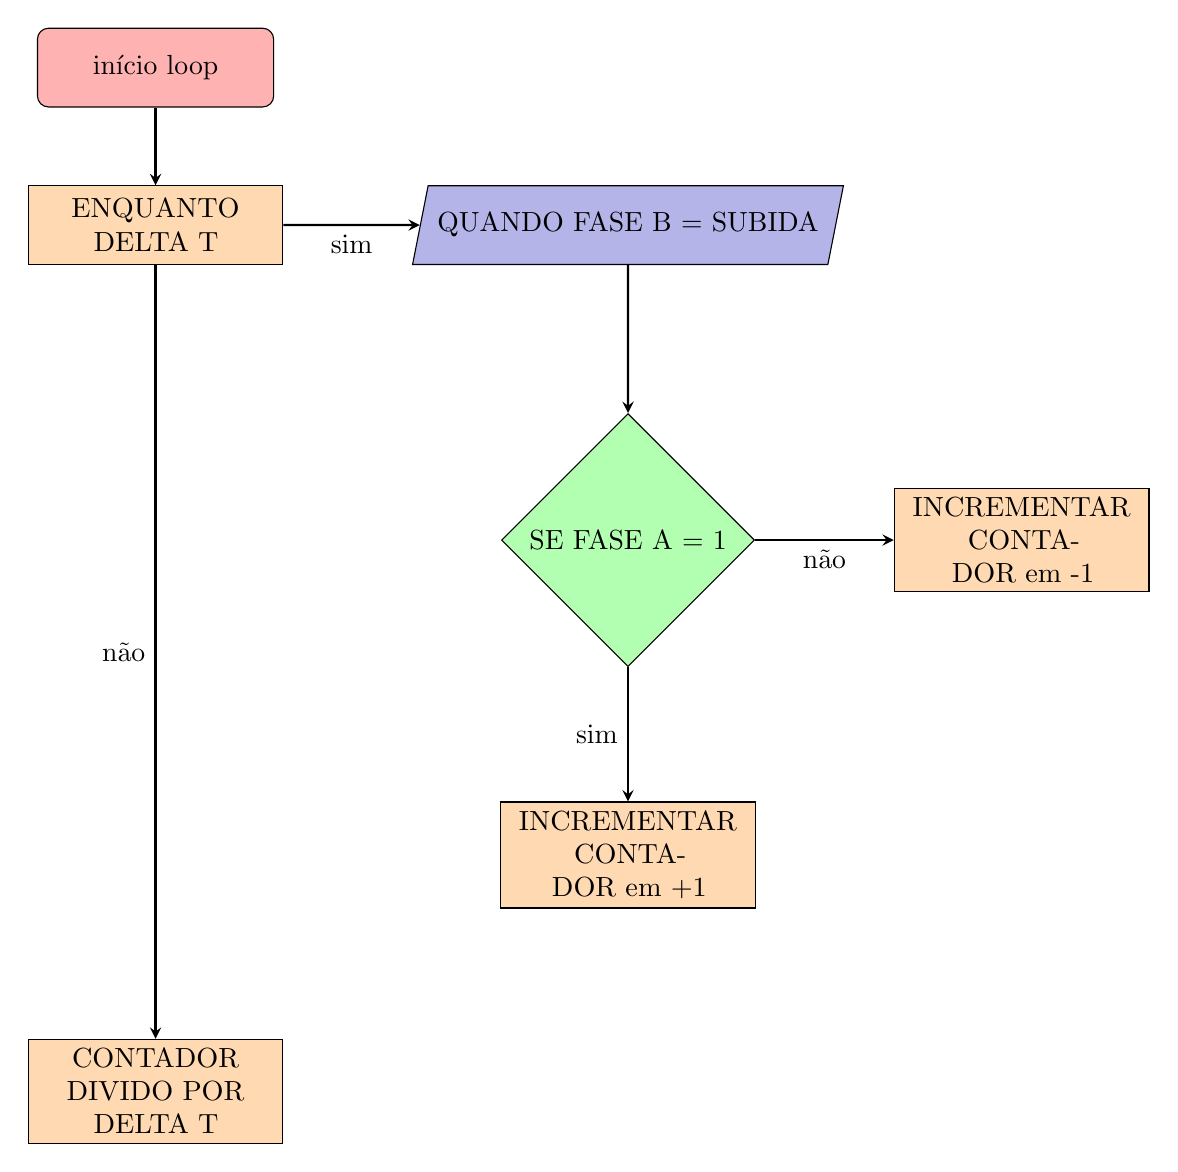
\begin{tikzpicture}[node distance=2cm]

    \node (start) [startstop] {início loop};
    \node (pro1) [process, below of=start] {ENQUANTO DELTA T};
    
    \node (in1) [io, right of=pro1, xshift= 4cm] {QUANDO FASE B = SUBIDA};
    
    \node (dec1) [decision, below of=in1, yshift=-2cm] {SE FASE A = 1};
    \node (pro1a) [process, below of=dec1, yshift= -2cm] {INCREMENTAR CONTADOR em +1};
    \node (pro1b) [process, right of=dec1, xshift= 3cm] {INCREMENTAR CONTADOR em -1};
    
    
    \node (count) [process, below of=pro1, yshift= -9cm] {CONTADOR DIVIDO POR DELTA T};
    
    \draw [arrow] (start) -- (pro1);
    \draw [arrow] (pro1) -- node[anchor=north] {sim} (in1);
    \draw [arrow] (in1) -- (dec1);
    \draw [arrow] (dec1) -- node[anchor=east] {sim} (pro1a);
    \draw [arrow] (dec1) -- node[anchor=north] {não} (pro1b);
    
    \draw [arrow] (pro1) -- node[anchor=east] {não} (count);

\end{tikzpicture}



Na implementação dessa lógica no STM32, o desafio foi a definição do $\Delta_{T}$,
Se o $\Delta_{T}$ for muito pequeno, o resultados de pulsos por segundo pode tender ao infinito, gerando valores muito altos.
Na figura \ref{fig:medidas_altas} em laranja, esta o resultado do rpm considerando o $\Delta_{T}$ como o tempo entre os ciclos do micrcontrolador.
A outra opção, foi definir um $\Delta_{T}$ fixo, definindo uma frequencia de medição pré definida, e o resultado pode ser visto em azul na figura \ref{fig:medidas_altas}
Essa outra opção de $\Delta_{T}$ resultou em um sinal que tem uma componente em alta frequência com uma amplitude até consideral.
Analisando os dois sinais no dominio da frequêcia na figura \ref{fig:frequencia_medidas_altas}, o espectro em frequência do sinal em laranja possui amplitudes muitos semelhante em todo espectro, mas o espectro do sinal em azul, fica bem claro que em altas frequencias é composto mais por ruidos
e as frequencia médias tem amplitude menor em relação as frequências baixas, o que torna mais fácil aplicar um filtro passa-baixa para reduzir as frenquências médias e altas.

A figura \autoref{passa_baixa_teste}, mostra um dos teste de filtro passa baixa, em o sinal em laranja ainda persiste esses valores tentendo ao infinito, devido a ampliture eles se tornam um pouco dificil de serem retirados.
Mas o sinal em azul acaba tendo um resultado melhor depois do filtro, muito semelhando ao sinal em laranja.
Com base nesse resultado, foi decidido seguir com o método em que o $\Delta_{T}$ é definido por uma frequência pré definida.


\begin{figure}[h]
    \centering
    \includegraphics{figures/medidas_altas}
    \caption{Problemas com delta T muito pequeno}
    \label{fig:medidas_altas}
\end{figure}

\begin{figure}[h]
    \centering
    \includegraphics{figures/frequencia_medidas_altas}
    \caption{Frequências}
    \label{fig:frequencia_medidas_altas}
\end{figure}

\begin{figure}[h]
    \centering
    \includegraphics{figures/passa_baixa_teste}
    \caption{Passa baixa teste}
    \label{fig:passa_baixa_teste}
\end{figure}


Com o método definido, foi definido um $\Delta_{T}$ em 100hz eu um filtro passa baixa em 2hz
As imagens no anexo \autoref{att_medicao_motores}, mostra as imagens comparando o sinal original e o sinal filtrado para cada motor.
A equação \autoref{eqn:equacao_diferenca} a seguir é a equação de diferença do filtro, considerando uma amostragem de 100hz e frequência de corte em 2hz.

\begin{equation}
    \begin{split}
        y[k] = 0.0591174 \cdot u \left[ k \right] +  0.0591174 \cdot u[k - 1] + 0.88176521 \cdot y[k - 1]
    \end{split}
    \label{eqn:equacao_diferenca}
\end{equation}

\subsubsection{Curva PWM x RPM - problema da não linearidade}

Depois de definido como calcular a velocidade o próximo desafio foi lidar com a não linearidade entre o PWM e o resultado medido em RPM.
Como pode ser visto na figura \autoref{grafico_pwm_x_rpm}, na comparação entre o valor do PWM e o RPM no tempo.

\begin{figure}[htb]
	\centering
	\includegraphics{figures/pwm_x_rpm}
	\caption{Curva PWM e RPM no tempo}
	\label{fig:grafico_pwm_x_rpm}
\end{figure}

Considerando essa não linearidade, foram realizadas 15k medições em PWM vs RPM para definir uma equação que pudesse relacionar o PWM com o RPM.
Como pode ser observado na figura  \autoref{medicao_pwm_x_rpm_dados_brutos}, os resultados possuem uma tendência, mas possuem alguns pontos fora da curta.
devido ao esses ruídos nas medições ss dados foram tratatos para obter valores médios dos resultados usando python,
o código pode ser visto no anexo \autoref{att_limpeza_python}.

\begin{figure}[htb]
	\centering
	\includegraphics{figures/curva_pwm_x_rpm_dados_brutos}
	\caption{Curva PWM x RPM dados brutos}
	\label{fig:medicao_pwm_x_rpm_dados_brutos}
\end{figure}


O resultado da limpeza dos dados pode ser vizualizado na figura \autoref{medicao_pwm_x_rpm_dados_medios}.
Após a limpeza dos dados, os dados foram importados para o matlab, anexo \autoref{att_matlab},
para obter um polinômio que possa definir a curva, o polinômio resultante é a equação \ref{eqn:polimonio_rpm}, e a figura \autoref{curva_ajustada} representa a curva ajustada.
A equação do polinômio foi inserida no código do micrcontrolador, foi testado definir um RPM de 150, e a tabela \autoref{medicao_motores} trás uma amostra dos resultados dos RPMs de cada motor.
Com essa equação é mais fácil definir um comportamento linear, facilitando a aplicação de um controle PDI.

\begin{equation}
    \begin{split}
        0.0001131x^{4} + -0.03064x^{3} + 2.993x^{2} + -1.257x + 9017
    \end{split}
    \label{eqn:polimonio_rpm}
\end{equation}

\begin{figure}[htb]
	\centering
	\includegraphics{figures/curva_pwm_x_rpm_dados_medios}
	\caption{Curva PWM x RPM dados médios}
	\label{fig:medicao_pwm_x_rpm_dados_medios}
\end{figure}

\begin{figure}[htb]
	\centering
	\includegraphics{figures/curva_ajustada}
	\caption{Curva ajustada}
	\label{fig:curva_ajustada}
\end{figure}



\begin{quadro}[htb]
	\caption{\label{medicao_motores}Medição rpms motores}
	 \begin{tabular}{|c|c|c|c|c|}
		\hline
		\textbf{$Tempo_{seg}$} & \textbf{$RPM_{definido}$} & \textbf{$RPM_{real_{1}}$} & \textbf{$RPM_{real_{2}}$} & \textbf{$RPM_{real_{3}}$} \\ \hline
		52.954 & 150.00  & 141.03 & 162.69 & 149.82 \\ \hline
		52.954 & 150.00  & 141.43 & 162.43 & 149.18 \\ \hline
		53.000 & 150.00  & 140.83 & 162.19 & 148.61 \\ \hline
		53.000 & 150.00  & 140.30 & 161.98 & 149.06 \\ \hline
		53.000 & 150.00  & 140.79 & 161.80 & 149.46 \\ \hline
		53.000 & 150.00  & 141.21 & 161.64 & 148.86 \\ \hline
		53.046 & 150.00  & 141.59 & 161.49 & 149.28 \\ \hline
		53.046 & 150.00  & 141.92 & 161.37 & 149.65 \\ \hline
		53.046 & 150.00  & 141.26 & 161.25 & 149.02 \\ \hline
		53.046 & 150.00  & 140.68 & 162.11 & 148.48 \\ \hline
		53.046 & 150.00  & 141.12 & 162.86 & 148.94 \\ \hline
		53.092 & 150.00  & 141.51 & 162.57 & 149.35 \\ \hline
		53.092 & 150.00  & 141.85 & 162.32 & 148.76 \\ \hline
		53.092 & 150.00  & 141.20 & 162.09 & 149.19 \\ \hline
		53.092 & 150.00  & 140.63 & 161.90 & 149.57 \\ \hline
	\end{tabular}
\end{quadro}


\subsection{Implementação da medição de rpm e filtro passa baixa no microcontrolador}

Para medir a velocidade de um motor DC com base no encoder, foi necessário realizar a leitura das subidas dos calores de LOW para HIGH de uma das fases do enconder, e comparar com outra Fase
Para isso usamos o sistema de interrupção do microcontrolador.
Exemplo do trecho de código que realiza a leitura dos valores do encoder, e registra em um contador a quantidade de pulsos de uma fase.


\lstset{language=C}
\begin{lstlisting}
long prevTime = 0;
long currTime = micros();
volatile int pos_i_1 = 0;
int prevPosition_1 = 0;
void setup() {
    motorsSetupPins(); encodersSetupPins();
    attachInterrupt(digitalPinToInterrupt(PB0), readEncoder1, RISING);
}
void loop() {
	int currPosition_1 = 0;
    ATOMIC_BLOCK(ATOMIC_RESTORESTATE){currPosition_1 = pos_i_1;};
    prevPosition_1 = currPosition_1;
}

void readEncoder1(){ 
    int b = digitalRead(PB1);
    if(b>0){pos_i_1++;}
    else {pos_i_1--;}
}
\end{lstlisting}


Após obtendo os a quantidade de pulsos é possivel calcular a taxa de pulsos por segundo, usando o diferencial da velocidade no dominio discreto, $\Delta$p/$\Delta$t.

\lstset{language=C}
\begin{lstlisting}
#define HALL_RESOLUTION 374
long prevTime = 0;
long currTime = micros();
volatile int pos_i_1 = 0;
int prevPosition_1 = 0;
float direction_angle = 90;
void setup() {
    motorsSetupPins();
    encodersSetupPins();
    attachInterrupt(digitalPinToInterrupt(PB0), readEncoder1, RISING);  
}
void loop() {
	currTime = micros();
	int currPosition_1 = 0;
	ATOMIC_BLOCK(ATOMIC_RESTORESTATE){currPosition_1 = pos_i_1;};
	float rpm1 = calc_rpm(currTime, prevTime, currPosition_1, prevPosition_1);
	prevPosition_1 = currPosition_1;
	prevPosition_3 = currPosition_3;
	prevTime = currTime;
}
void readEncoder1(){ 
    int b = digitalRead(PB1);
    if(b>0){pos_i_1++;}
    else {pos_i_1--;}
}
float calc_rpm(long currT, long prevT, int pos, int posPrev){
    float deltaT = ((float) (currT-prevT))/1.0e6;
    float pulse_per_seconds = (pos - posPrev)/deltaT;
    float rpm = 60*pulse_per_seconds/HALL_RESOLUTION;
    return rpm;
}
\end{lstlisting}


Porém calcular velocidade a cada ciclo do micrcontrolador acaba registrando valores de tempo muito pequenos, fazendo a velocidade tender ao infinito
A solução foi estabelecer uma amostragem do registro da velocidade, porem a amostragem adiciona um ruido com frequências maiories que do sinal original e de amplitude definida.
Para retirar essas frequência do sinal, o filtro passa baixa foi implementado no código.


\lstset{language=C}
\begin{lstlisting}
#define HALL_RESOLUTION 374
#define DT_TIME_SAMPLE_RATE_ENCODER 10 // encoder position reading update rate
int nextChangeSampleRate  = (millis() + DT_TIME_SAMPLE_RATE_ENCODER);
long prevTime = 0;
long currTime = micros();
volatile int pos_i_1 = 0;
int prevPosition_1 = 0;
float filterRpm_1 = 0;
float prevRpm_1 = 0;
void setup() {
    encodersSetupPins();
    attachInterrupt(digitalPinToInterrupt(PB0), readEncoder1, RISING);   
}

void loop() {
    if (millis()>=nextChangeSampleRate){
        currTime = micros();
        int currPosition_1 = 0;
        ATOMIC_BLOCK(ATOMIC_RESTORESTATE){currPosition_1 = pos_i_1;};
        float rpm1 = calc_rpm(currTime, prevTime, currPosition_1, prevPosition_1);
        filterRpm_1 = low_pass_filter_first_order(rpm1, prevRpm_1, filterRpm_1);
        prevPosition_1 = currPosition_1;
        prevRpm_1 = rpm1;
        prevTime = currTime;
        nextChangeSampleRate = millis() + DT_TIME_SAMPLE_RATE_ENCODER;
    }
}
void readEncoder1(){ 
    int b = digitalRead(PB1);
    if(b>0){pos_i_1++;}
    else {pos_i_1--;}
}
float calc_rpm(long currT, long prevT, int pos, int posPrev){
    float deltaT = ((float) (currT-prevT))/1.0e6;
    float pulse_per_seconds = (pos - posPrev)/deltaT;
    float rpm = 60*pulse_per_seconds/HALL_RESOLUTION;
    return rpm;
}
float low_pass_filter_first_order(float currRpm, float prevRpm, float prevFilterRpm){
    float posFilterRpm = 0.881765*prevFilterRpm + 0.0591174*currRpm + 0.0591174*prevRpm;
    return posFilterRpm;
}
\end{lstlisting}

\subsection{Motores de passo}

\lipsum[1]




%https://www.aarohies.com/what-is-the-difference-between-pmdc-bldc-and-pmsm-motor/
%https://www.monolithicpower.com/en/learning/resources/brushless-vs-brushed-dc-motors
%https://techweb.rohm.com/product/motor/brushed-motor/209/

\section{Drivers}

\lipsum[1]

\section{Alimentação}


\subsection{Microcontrolador}

Para ambos os microcontroladores testados, STM32 e ESP32,
podem ser usados os pinos de 5v  e 3.3v e a porta micro-USB-B

\subsubsubsection{Pino de 5v não regulado}

Para o ESP32, fontes divergem em relação à tensão mínima e máxima 
que pode ser usada, porém, a maioria concorda em manter de
6v a 7v \cite{esp32_reference_power_supply_1,esp32_reference_power_supply_2, esp32_reference_2}.
Para o STM32 não se encontra informações que discutam o limite máximo de tensão no pino, mas segundo \cite{stm_doc},
o recomendado é manter em 5v.

\subsubsubsection{Pino de 3.3v regulado}
Em ambos as placas, esse pino é mais sensível a variações, pois esta em curto com a alimentação
dos chips, então o ideal é manter entre 3.1v e 3.3v.

\subsubsubsection{Micro-USB-B}
Essa opção permite usar um powerbank, porém o conector das placas é um Micro-USB-B,
modelo que usa protocolo USB 2.0, que pode fornece apenas a 500mA a 5v \cite{micro_usb_b}.
500mA É suficiente para alimentar o ESP32 e o STM32, que podem consumir 
até 260mA \cite{esp_max_current} e 150mA \cite{stm32_datasheet}, respectivamente.

Porem um powerbank pode ser uma solução muito ineficiente do ponto de vista energético,
os modelos populares possuem baterias de lítio de 3.7v, essa tensão é convertido para 5v,
e posteriormente dentro do ESP32 é convertida novamente para 3.3v
No modelo PN-952 da CNHPineng sai de 5000mAh a 3.7v  para 3160mAh a 5v,
podendo novamente perder mais corrente por hora ao ser convertido para 3.3v no ESP32.


\subsection{Motores DC}
Para os motores DC, de 6v, uma bateria de chumbo-ácido de 6v 4,5Ah, 
comumente usada em sistema de câmeras de segurança,
alarmes e iluminação de emergência \cite{bateria_6v_ref_1,bateria_6v_ref_2}.

\begin{figure}[ht]
	\centering
	\caption{Bateria selada de chumbo 6V 4,5Ah}
	\includegraphics[width=0.4\textwidth]{figures/bateria_6v}
    \caption*{FONTE: Grupo Elgin}
	\label{bateria_6v}
\end{figure}

\subsection{Motores de passo}

Os motores de passo NEMA 17 podem ser alimentados, através do driver, com 12v a 24v.
Observando a possibilidade de uma bateria de 12v/24v ficar sem uso depois do projeto,
e considerando que ferramentas elétricas possuem baterias padronizadas de 12v/18v/36V, 
foi considerando utilizar 3 baterias de 12v da bosch, que já estavam disponíveis para uso.
Cada bateria tem tensão nominal de 12v a 2Ah, do modelo GBA, 
são usadas em aspirador de pó, esmerilhadeiras, furadeiras, plainas e serras circulares.
Conforme as instruções do pacote da bateria tem pico máximo de carga 12v, porém em uso a bateria possui 10.8v,
pois é fabricada com 3 células de 3.6v
Durante os testes com os motores NEMA 17,  as baterias apresentam uma tensão variando de 10.6 a 10.7
Como essas baterias já haviam sido adquiridas antes desse projeto para uso pessoal,
usá-las no projeto se tornou uma opção economicamente viável e sustentável,
já que as baterias ainda usadas em ferramentas pessoais.

\begin{figure}[ht]
	\centering
	\caption{Bateria de ions de litio - Bosch GBA 12v 2Ah}
	\includegraphics[width=0.25\textwidth]{figures/gba_bosch_bateria}
    \caption*{FONTE: BOSCH loja Online}
	\label{gba_bosch_bateria}
\end{figure}


\begin{figure}[ht]
	\centering
	\caption{Parte de trás da embalagem da bateria Bosch GBA 12v}
	\includegraphics[width=0.8\textwidth]{figures/gba_bosch_embalagem}
    \caption*{FONTE: BOSCH loja Online}
	\label{gba_bosch_embalagem}
\end{figure}

Porém usar essas baterias traz um desafio diferente, a instalação.  Esse tópico é discutido na seção \ref{secao_fabricacao}.


\chapter{Fabricação e montagem}

\section{CAD}

blabla

\begin{figure}[h]
	\centering
	\includegraphics{figures/cad1}
	\caption{Base do robô}
	\label{fig:base_robo}
\end{figure}

\begin{figure}[h]
	\centering
	\includegraphics{figures/cad2}
	\caption{Suporte Protoboard}
	\label{fig:suport_protoboard}
\end{figure}

\begin{figure}[h]
	\centering
	\includegraphics{figures/cad3}
	\caption{Mancais dos Motores - 1}
	\label{fig:mancais}
\end{figure}

\begin{figure}[h]
	\centering
	\includegraphics{figures/cad3_2}
	\caption{Mancais dos Motores - 2}
	\label{fig:mancais_2}
\end{figure}

\begin{figure}[h]
	\centering
	\includegraphics{figures/cad4}
	\caption{peça que conecta o suporte de protoboard e a base - 1}
	\label{fig:peca_juncao}
\end{figure}

\begin{figure}[h]
	\centering
	\includegraphics{figures/cad4_2}
	\caption{peça que conecta o suporte de protoboard e a base - 2}
	\label{fig:peca_juncao_2}
\end{figure}



\section{modelagem 3D}

blabla

\begin{figure}[h]
	\centering
	\includegraphics{figures/3d_1}
	\caption{Modelagem 3d da base do robô}
	\label{fig:base_robo_3d}
\end{figure}

\begin{figure}[h]
	\centering
	\includegraphics{figures/3d_2}
	\caption{Modelagem 3d do suporte do protoboard}
	\label{fig:suport_protoboard_3d}
\end{figure}

\begin{figure}[h]
	\centering
	\includegraphics{figures/3d_3}
	\caption{Modelagem 3d dos mancais}
	\label{fig:mancais_3d}
\end{figure}

\begin{figure}[h]
	\centering
	\includegraphics{figures/3d_4}
	\caption{Modelagem 3d peça de junção}
	\label{fig:peca_juncao_3d}
\end{figure}


\section{Impressão e montagem}

\begin{figure}[h]
	\centering
	\includegraphics{figures/impressao}
	\caption{Impressão das peças}
	\label{fig:impressao}
\end{figure}

\begin{figure}[h]
	\centering
	\includegraphics{figures/montagem_1}
	\caption{Montagem 1}
	\label{fig:montagem}
\end{figure}

\begin{figure}[h]
	\centering
	\includegraphics{figures/montagem_2}
	\caption{Montagem 2}
	\label{fig:montagem_2}
\end{figure}

\begin{figure}[h]
	\centering
	\includegraphics{figures/montagem_3}
	\caption{Montagem 3}
	\label{fig:montagem_3}
\end{figure}


\begin{figure}[h]
	\centering
	\includegraphics{figures/montagem_4}
	\caption{Testes dos motores}
	\label{fig:montagem_4}
\end{figure}


\section{Controle e comunicação com o microcontrolador}

\lipsum[1]

\section{Segurança}

\lipsum[1]

	
	

\chapter{Resultados e Discussão}

\lipsum[1]
	
	% ----------------------------------------------------------
	% Finaliza a parte no bookmark do PDF
	% para que se inicie o bookmark na raiz
	% e adiciona espaço de parte no Sumário
	% ----------------------------------------------------------
	\phantompart

% ELEMENTOS PÓS-TEXTUAIS
\postextual

	% Referências bibliográficas

	\bibliography{bibliography/bibliografia.bib}
	%\printbibliography


	% Glossário
	%\input{glossary/glossary_class.tex}

	% Apêndices
	%\begin{apendicesenv}

% Imprime uma página indicando o início dos apêndices
\partapendices


\chapter{apendice 1}


\lipsum[1]

\chapter{apendice 2}

\lipsum[1]


\end{apendicesenv}

	% Anexos
	% \begin{anexosenv}
	% \partanexos
	% \chapter{Medição de velocidade dos motores}
\label{att_medicao_motores}

\begin{figure}[h]
	\centering
	\includegraphics{figures/explicacao_quadros}
	\caption{Explicação de cada quadro nas figuras a seguir}
	\label{fig:explicacao_quadros}
\end{figure}


\begin{figure}[h]
	\centering
	\includegraphics{figures/medidas_motor_1}
	\caption{Medidas Motor 1}
	\label{fig:medidas_motor_1}
\end{figure}

\begin{figure}[h]
	\centering
	\includegraphics{figures/medidas_motor_2}
	\caption{Medidas Motor 2}
	\label{fig:medidas_motor_2}
\end{figure}


\begin{figure}[h]
	\centering
	\includegraphics{figures/medidas_motor_3}
	\caption{Medidas Motor 3}
	\label{fig:medidas_motor_3}
\end{figure}




	% 

\chapter{Filtro passa baixa de primeira ordem}

Tranformação da função de transferncia para domínio discreto usando o método bilinear.

\begin{equation}
    \begin{split}
        H\left( s \right) = \frac{\omega_c}{s + \omega_c} = 
        \frac{1}{1 + \frac{s}{\omega_c}}
        =  \frac{Y \left( s \right)}{ U \left( s \right)}
    \end{split}
\end{equation}

\begin{equation}
    \begin{split}
        z = \frac{2}{T_s}\frac{z-1}{z+1}
    \end{split}
\end{equation}

\begin{equation}
    \begin{split}
        f=2Hz
    \end{split}
\end{equation}

\begin{equation}
    \begin{split}
        Ts=1/100
    \end{split}
\end{equation}

\begin{equation}
    \begin{split}
        \omega_c = 2 \pi f
    \end{split}
\end{equation}


\begin{equation*}
    \begin{split}
        \frac{1}{1 + \frac{s}{\omega_c}}
        = \frac{1}{1 + \frac{2}{T_s\omega_c}\frac{z-1}{z+1}} 
        = \frac{z + 1}{z + 1 + \left( z-1 \right) \frac{2}{T_s\omega_c}} \\
        = \frac{1 + z^{-1}}{1 + z^{-1} + \left( 1 - z^{-1} \right) \frac{2}{T_s\omega_c}}
        = \frac{\left(1 + z^{-1} \right) \frac{T_s\omega_c}{2} }{\left(1 + z^{-1} \right) \frac{T_s\omega_c}{2} +  1 - z^{-1} } \\
        = \frac{\left(1 + z^{-1} \right) \frac{T_s\omega_c}{2} }
        { \left(\frac{T_s\omega_c}{2} + 1 \right) + \left(\frac{T_s\omega_c}{2} - 1 \right) z^{-1} }
        = \frac{\left(1 + z^{-1} \right) \frac{T_s\omega_c}{2} \left( \frac{2}{T_s\omega_c + 2} \right) }
        { 1 + \left( \frac{2}{T_s\omega_c + 2} \right) \left(\frac{T_s\omega_c}{2} - 1 \right) z^{-1} }
    \end{split}
\end{equation*}


\begin{equation}
    \begin{split}
        H\left( s \right) = \frac{\left(1 + z^{-1} \right) \frac{T_s\omega_c}{T_s\omega_c + 2}  }
        { 1 + \left( \frac{T_s\omega_c - 2}{T_s\omega_c + 2} \right) z^{-1} }
    \end{split}
\end{equation}


\begin{equation*}
    \begin{split}
        = \frac{\left(1 + z^{-1} \right) \frac{0.01 \cdot 2 \pi f }{0.01 \cdot 2 \pi f + 2}  }
        { 1 + \left( \frac{0.01 \cdot 2 \pi f - 2}{0.01 \cdot 2 \pi f + 2} \right) z^{-1} }
    \end{split}
\end{equation*}

\begin{equation*}
    \begin{split}
        = \frac{\left(1 + z^{-1} \right) \frac{0.04 \pi}{0.04 \pi + 2}  }
        { 1 + \left( \frac{0.04 \pi - 2}{0.04 \pi + 2} \right) z^{-1} }
    \end{split}
\end{equation*}

\begin{equation}
    \begin{split}
        \frac{Y \left( z \right)}{ U \left( z \right)} = \frac{ 0.0591174 + 0.0591174 z^{-1} }
        { 1 - 0.88176521 z^{-1} }
    \end{split}
\end{equation} 

Obtendo a equação de diferença a ser usada no microcontrolador.

\begin{equation*}
    \begin{split}
        U \left( z \right) 0.0591174 +  U \left( z \right) 0.0591174 z^{-1}
        =  Y \left( z \right) - Y \left( z \right) 0.88176521 z^{-1}
    \end{split}
\end{equation*} 

\begin{equation}
        \begin{split}
            X \left( z \right) = x[k] \\
            X \left( z \right) z^{-1} = x[k - 1] \\
        \end{split}
\end{equation}


\begin{equation}
    \begin{split}
        y[k] = 0.0591174 \cdot u \left[ k \right] +  0.0591174 \cdot u[k - 1] + 0.88176521 \cdot y[k - 1]
    \end{split}
\end{equation}
	% \chapter{Fabricação e montagem}

\section{CAD}

blabla

\begin{figure}[h]
	\centering
	\includegraphics{figures/cad1}
	\caption{Base do robô}
	\label{fig:base_robo}
\end{figure}

\begin{figure}[h]
	\centering
	\includegraphics{figures/cad2}
	\caption{Suporte Protoboard}
	\label{fig:suport_protoboard}
\end{figure}

\begin{figure}[h]
	\centering
	\includegraphics{figures/cad3}
	\caption{Mancais dos Motores - 1}
	\label{fig:mancais}
\end{figure}

\begin{figure}[h]
	\centering
	\includegraphics{figures/cad3_2}
	\caption{Mancais dos Motores - 2}
	\label{fig:mancais_2}
\end{figure}

\begin{figure}[h]
	\centering
	\includegraphics{figures/cad4}
	\caption{peça que conecta o suporte de protoboard e a base - 1}
	\label{fig:peca_juncao}
\end{figure}

\begin{figure}[h]
	\centering
	\includegraphics{figures/cad4_2}
	\caption{peça que conecta o suporte de protoboard e a base - 2}
	\label{fig:peca_juncao_2}
\end{figure}



\section{modelagem 3D}

blabla

\begin{figure}[h]
	\centering
	\includegraphics{figures/3d_1}
	\caption{Modelagem 3d da base do robô}
	\label{fig:base_robo_3d}
\end{figure}

\begin{figure}[h]
	\centering
	\includegraphics{figures/3d_2}
	\caption{Modelagem 3d do suporte do protoboard}
	\label{fig:suport_protoboard_3d}
\end{figure}

\begin{figure}[h]
	\centering
	\includegraphics{figures/3d_3}
	\caption{Modelagem 3d dos mancais}
	\label{fig:mancais_3d}
\end{figure}

\begin{figure}[h]
	\centering
	\includegraphics{figures/3d_4}
	\caption{Modelagem 3d peça de junção}
	\label{fig:peca_juncao_3d}
\end{figure}


\section{Impressão e montagem}

\begin{figure}[h]
	\centering
	\includegraphics{figures/impressao}
	\caption{Impressão das peças}
	\label{fig:impressao}
\end{figure}

\begin{figure}[h]
	\centering
	\includegraphics{figures/montagem_1}
	\caption{Montagem 1}
	\label{fig:montagem}
\end{figure}

\begin{figure}[h]
	\centering
	\includegraphics{figures/montagem_2}
	\caption{Montagem 2}
	\label{fig:montagem_2}
\end{figure}

\begin{figure}[h]
	\centering
	\includegraphics{figures/montagem_3}
	\caption{Montagem 3}
	\label{fig:montagem_3}
\end{figure}


\begin{figure}[h]
	\centering
	\includegraphics{figures/montagem_4}
	\caption{Testes dos motores}
	\label{fig:montagem_4}
\end{figure}

	% \chapter{Limpeza dos dados realizada no python}
\label{att_limpeza_python}


\lstset{language=Python}
\begin{lstlisting}
    import json
    import pandas as pd
    import numpy as np
    import matplotlib.pyplot as plt
    
    res = open('medidas_capturadas.txt').read()
    res = res.split('\n')
    
    res = [json.loads(i[i.find('''{"millis":'''):]) for i in res]
    
    dados_brutos = pd.DataFrame(res)
    
    dados_brutos = pd.concat([
        dados_brutos[['w1','filterRpm_1']]
        .rename(columns={'filterRpm_1':'filter_rpm_','w1':'w'}),
        dados_brutos[['w2','filterRpm_2']]
        .rename(columns={'filterRpm_2':'filter_rpm_','w2':'w'}),
        dados_brutos[['w3','filterRpm_3']]
        .rename(columns={'filterRpm_3':'filter_rpm_','w3':'w'})
    ]).sort_values('w')
    
    
    dados_medios = dados_brutos.groupby('w').agg({
        'filter_rpm_':['mean']
    }).reset_index()
    
    
    dados_medios.columns = [''.join(i) for i in dados_medios.columns]
    
    dados_medios['cut'] = (dados_medios['w']/200).astype(int)
    dados_medios_amostra = dados_medios.groupby('cut').first().reset_index()
    
    dados_medios_amostra[
        ['filter_rpm_mean', 'w']
    ].to_csv('amostra_invertida.csv', index=False)

\end{lstlisting}

	% \chapter{Limpeza dos dados realizada no python}
\label{att_matlab}

Matlab
\lstset{language=Matlab}
\begin{lstlisting}
    T = readtable('amostra_invertida.csv');
    filter_rpm_mean =  T{:,1};
    w =  T{:,2};
    f=fit(filter_rpm_mean,w,'poly4')

    f = 
    
         Linear model Poly4:
         f(x) = p1*x^4 + p2*x^3 + p3*x^2 + p4*x + p5
         Coefficients (with 0.95 confidence bounds):
           p1 =   0.0001131  (9.732e-05, 0.0001288)
           p2 =    -0.03064  (-0.0375, -0.02377)
           p3 =       2.993  (1.999, 3.988)
           p4 =      -1.257  (-54.15, 51.63)
           p5 =        9017  (8235, 9798)

\end{lstlisting}
	% \end{anexosenv}


	

%---------------------------------------------------------------------
% INDICE REMISSIVO
%---------------------------------------------------------------------
\phantompart
\printindex


\end{document}

